\documentclass[11pt,letterpaper]{article}
\usepackage[lmargin=1in,rmargin=1in,tmargin=1in,bmargin=1in]{geometry}
\usepackage{../style/homework}
\usepackage{../style/commands}
\setbool{quotetype}{false} % True: Side; False: Under
\setbool{hideans}{true} % Student: True; Instructor: False

% -------------------
% Content
% -------------------
\begin{document}

\homework{5: Due 10/08}{The economy stinks, bees are dying, and movies are pretty much all sequels now.}{Winston Saint-Marie Schmidt, New Girl}


% Problem
\problem{10} Determine if the relations $f(x)$ and $g(x)$ shown below are functions. Explain why or why not. 
	\[
	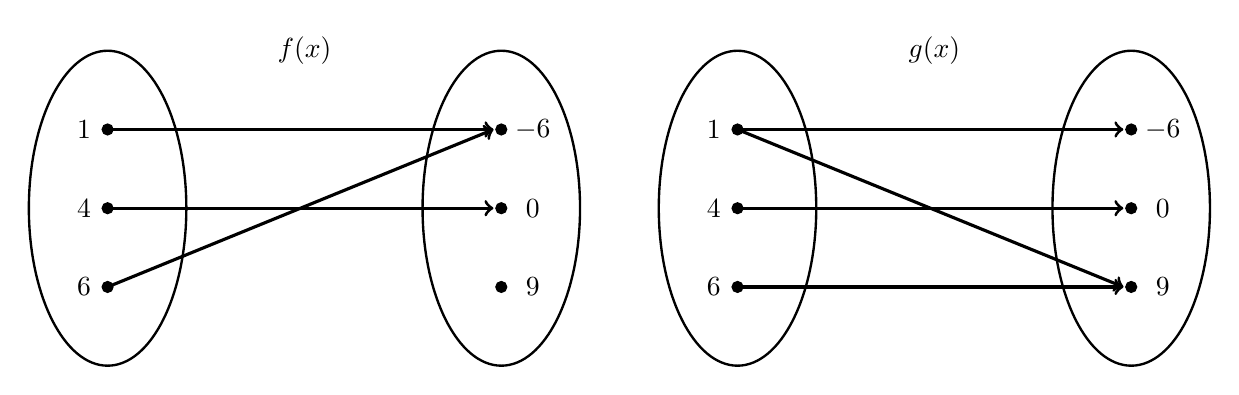
\begin{tikzpicture}
	\node at (2.5,2) {$f(x)$};
	% Ellipses
	\draw[line width=0.03cm] (0,0) circle (1 and 2);
	\draw[line width=0.03cm] (5,0) circle (1 and 2);
	
	% Nodes
	\draw[fill=black] (0,1) circle (0.07);
	\draw[fill=black] (0,0) circle (0.07);
	\draw[fill=black] (0,-1) circle (0.07);
	
	\draw[fill=black] (5,1) circle (0.07);
	\draw[fill=black] (5,0) circle (0.07);
	\draw[fill=black] (5,-1) circle (0.07);
	
	% Arrow
	\draw[line width=0.04cm,->] (0,1) -- (4.9,1);
	\draw[line width=0.04cm,->] (0,0) -- (4.9,0);
	\draw[line width=0.04cm,->] (0,-1) -- (4.9,1);
	
	% Labels
	\node at (-0.3,1) {$1$};
	\node at (-0.3,0) {$4$};
	\node at (-0.3,-1) {$6$};
	
	\node at (5.4,1) {$-6$};
	\node at (5.4,0) {$0$};
	\node at (5.4,-1) {$9$};
	
	\tikzset{shift={(8,0)}}
	%
	\node at (2.5,2) {$g(x)$};
	% Ellipses
	\draw[line width=0.03cm] (0,0) circle (1 and 2);
	\draw[line width=0.03cm] (5,0) circle (1 and 2);
	
	% Nodes
	\draw[fill=black] (0,1) circle (0.07);
	\draw[fill=black] (0,0) circle (0.07);
	\draw[fill=black] (0,-1) circle (0.07);
	
	\draw[fill=black] (5,1) circle (0.07);
	\draw[fill=black] (5,0) circle (0.07);
	\draw[fill=black] (5,-1) circle (0.07);
	
	% Arrow
	\draw[line width=0.04cm,->] (0,1) -- (4.9,1);
	\draw[line width=0.04cm,->] (0,1) -- (4.9,-1);
	\draw[line width=0.04cm,->] (0,0) -- (4.9,0);
	\draw[line width=0.04cm,->] (0,-1) -- (4.9,-1);
	
	% Labels
	\node at (-0.3,1) {$1$};
	\node at (-0.3,0) {$4$};
	\node at (-0.3,-1) {$6$};
	
	\node at (5.4,1) {$-6$};
	\node at (5.4,0) {$0$};
	\node at (5.4,-1) {$9$};
	\end{tikzpicture}
	\]



\newpage



% Problem
\problem{10} Determine if the relations $f(x)$ and $g(x)$ shown below are functions. Explain why or why not. 
	\begin{table}[!ht]
	\centering
	\begin{tabular}{c|rcc|r}
	$x$ & $f(x)$ & \hspace{1cm} & $x$ & $g(x)$ \\ \cline{1-2} \cline{4-5}
	$1$ & $8$ & & $5$ & $2$ \\
	$2$ & $-7$ & & $6$ & $\pi$ \\
	$3$ & $8$ & & $8$ & $1.87$ \\
	$4$ & $8$ & & $9$ & $-9$ \\
	$5$ & $10$ & & $5$ & $3$
	\end{tabular}
	\end{table}



\newpage



% Problem
\problem{10} Determine if the relations $f(x)$ and $g(x)$ shown below are functions. Explain why or why not. 
	\[
	\begin{aligned}
	f(x)&= 2.54x + 91 \\[0.3cm]
	g(x)&= x^3 - x + 1
	\end{aligned}
	\]



\newpage



% Problem
\problem{10} Suppose $f(x)$ is the function given below.
	\[
	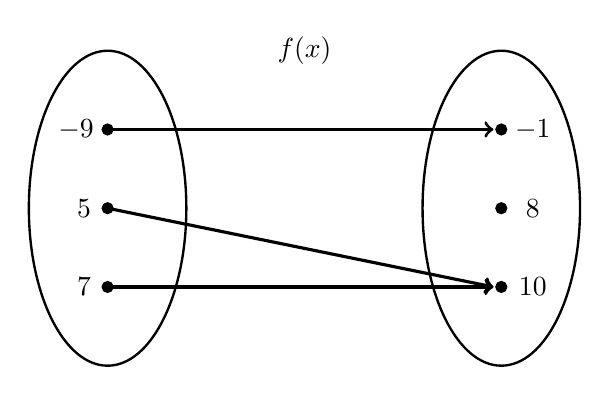
\begin{tikzpicture}
	\node at (2.5,2) {$f(x)$};
	% Ellipses
	\draw[line width=0.03cm] (0,0) circle (1 and 2);
	\draw[line width=0.03cm] (5,0) circle (1 and 2);
	
	% Nodes
	\draw[fill=black] (0,1) circle (0.07);
	\draw[fill=black] (0,0) circle (0.07);
	\draw[fill=black] (0,-1) circle (0.07);
	
	\draw[fill=black] (5,1) circle (0.07);
	\draw[fill=black] (5,0) circle (0.07);
	\draw[fill=black] (5,-1) circle (0.07);
	
	% Arrow
	\draw[line width=0.04cm,->] (0,1) -- (4.9,1);
	\draw[line width=0.04cm,->] (0,0) -- (4.9,-1);
	\draw[line width=0.04cm,->] (0,-1) -- (4.9,-1);
	
	% Labels
	\node at (-0.4,1) {$-9$};
	\node at (-0.3,0) {$5$};
	\node at (-0.3,-1) {$7$};
	
	\node at (5.4,1) {$-1$};
	\node at (5.4,0) {$8$};
	\node at (5.4,-1) {$10$};
	\end{tikzpicture}
	\]

\begin{enumerate}[(a)]
\item What is the domain of $f(x)$?
\item What is the codomain of $f(x)$?
\item What is the range of $f(x)$?
\end{enumerate}



\newpage



% Problem
\problem{10} Suppose $f(x)$ and $g(x)$ are the functions given below. 
        \begin{table}[!ht]
        \centering
        \begin{tabular}{| c || c | c | c | c | c | c | c |} \hline
	$x$ & $-2$ & $0$ & $1$ & $3$ & $4$ & $5$ & $10$ \\ \hline
	$f(x)$ & $5$ & $-3.1$ & $\pi$ & $5$ & $3/2$ & $14$ & $0$ \\ \hline
	$g(x)$ & $6$ & $4$ & $6.6$ & $-15$ & $4$ & $9$ & $2$ \\ \hline
        \end{tabular}
        \end{table}


Compute the following: \pspace
        \begin{enumerate}[(a)]
        \item $f(1)=$ \vfill
        \item $g(0)=$ \vfill
        \item $(f + g)(5)=$ \vfill
        \item $(f - g)(-2)=$ \vfill
        \item $(6f)(1)=$ \vfill
        \item $\left(\dfrac{f}{g}\right)(10)=$ \vfill
        \item $f(4)\, g(5)=$ \vfill
        \item $f(2 - g(0))=$ \vfill
        \item $(f \circ g)(0)=$ \vfill
        \item $(g \circ f)(3)=$ \vfill
        \end{enumerate}



\newpage



% Problem
\problem{10} Suppose $f(x)$ and $g(x)$ are the functions given below. 
	\[
	\begin{aligned}
	f(x)&= 3x - 1 \\[0.3cm]
	g(x)&= x^2 + x + 1
	\end{aligned}
	\]

Compute the following: \pspace
\begin{enumerate}[(a)]
\item $f(1)=$ \vfill
\item $g(0)=$ \vfill
\item $f(1) - 2g(1)=$ \vfill
\item $f(x) - g(x)=$ \vfill
\item $f(x) \, g(x)=$ \vfill
\item $\left( \dfrac{f}{g} \right)(x)=$ \vfill
\item $(g \circ f)(1)=$ \vfill
\item $f(g(0))=$ \vfill
\item $(f \circ g)(x)=$ \vfill
\item $(g \circ f)(x)=$ \vfill
\end{enumerate}










%\printpoints
\end{document}